% !BIB program = biber

\documentclass[12pt,a4 paper,title page]{article}
\usepackage[utf8]{inputenc}
\usepackage{microtype}
\usepackage[british]{datetime2} % For urldate formatting
\usepackage{natbib}
\usepackage{bibentry}

\usepackage{graphicx}
\usepackage{float}
\usepackage{textcomp}
\usepackage{xcolor}
\usepackage{soul,color}
\usepackage{colortbl}
\usepackage{amsthm}
\usepackage{bm}
\usepackage{algorithm}
\usepackage{algorithmic}
\usepackage{amsmath,amssymb,amsfonts}
\usepackage{svg}
\usepackage{array}
\usepackage{tabularx}
\usepackage[nottoc,notlot,notlof]{tocbibind}

\theoremstyle{definition}
\newtheorem{definition}{Definition}[section]
% \renewcommand{\algorithmicrequire}{ \textbf{Input:}} %Use Input in the format of Algorithm  
% \renewcommand{\algorithmicensure}{ \textbf{Output:}} %UseOutput in the format of Algorithm 

\usepackage[colorlinks = true,
            linkcolor = teal,
            urlcolor  = teal,
            citecolor = blue,
            anchorcolor = blue]{hyperref}
\usepackage{wrapfig}



\bibliographystyle{uts} % Import Harvard UTS style
\setcitestyle{aysep={}} % Remove comma separation between author and year for in-text citations
% \newcommand{\enquote}[1]{``#1''}

\title{Research Proposal: Adaptive Recommender System with Knowledge Graph}
\author{\large\textbf{Di Zhang}, \\
\textbf{supervisor: Professor Guangquan Zhang}, \\
\textbf{co-supervisor: Professor Jie Lu, Dr. Qian Zhang}, \\
\textbf{Student number: 31292711}}

\date{\Large{\textbf{Aug 2020}}}

\begin{document}
\sloppy
\maketitle

\tableofcontents
\newpage

\section*{Abstract}
Recommender systems are in high demand across various industries. Its results and effectiveness have been proven in e-commerce, entertainment, advertising, and many other business domains.
On the other hand, bringing a recommender system to market commonly faces data sparsity and cold start problems, which, further effects recommendation quality and sets a limit on predictions. 
Although lots of research effort has been devoted to developing algorithms in tackling the issues as mentioned above, we have not yet seen a framework that solves the data and model capacity challenges in a holistic approach.
In this research, we combine representation embedding and cross-domain transfer learning techniques on top of knowledge graph to form a unified framework. The framework enhances data and model prediction capability in an end-to-end schema. The result would significantly improve the recommendation model performance in sparse or foreign data conditions. 
The research aims to ease the barrier of launching recommender systems, hence promote its business adoption to a broader audience. 
This research is aim to answer the following questions:
1) How to represent users and items in a unified heterogeneous knowledge graph for improving data density?
2) How to improve recommender systems' adaptiveness on new and unseen data with knowledge graph embedding?
3) How to use knowledge graphs to transfer cross-domain knowledge for enhanced recommendation results?
Finally, research will conduct a recommender system case study to validate and proposed methods.

\subsection*{Keywords} 
Recommender System, Heterogeneous Information Network, Knowledge Graph, Transfer Learning.

%!TEX root = main.tex

\section*{Abstracts}
T.B.D.

\subsection*{Keywords} 
Recommender system, Heterogeneous Information Network, Knowledge Graph, Transfer Learning, Feature Representation Learning

\section{Introduction and background}
Recommender System (RS) is an indispensable technology, it evolves around our everyday life on multiple fronts. RS help us to find personalized interests from information overloads \citep{Lu2015}. It can act as a decision assisting agents to simplify or accelerate decision making process. Further more, as we experiencing the exponential growth of data content, RS keeps us updated on new emerging information.
Over the years, we see RS being adopted across different industries. At the same time, we noticed that, bringing a recommender systems into real-world application often faces many different sorts of challenges. 

Recommender systems exists long before computer was invented. Catalogs can be considered a one of the most primitive content-based recommender systems. In 2006, 100 million datasets were released by Netflix \citep{Bennett2007} The action expedited the research on Collaborative Filtering (CF). Over decades, Matrix Factorization based approach is still at the forefront of Recommender systems Field. Many new approaches and extensions had been evolved based on Collaborative Filtering to tackle its computation challenges and data sparsity problems. 

Transfer Learning \citep{Pan2010} in Cross Domain recommender system is another promising area which allowing recommendation possible in when initial user interaction data is scarce in target domains. \citet{Elkahky2015} experimented this approach on multiple Microsoft products, and concluded multi domain recommender system significantly outperforms single domain recommender systems. 


Meanwhile, building recommender system requires systematic approach, beyond algorithm and statistical analytics. Being overwhelmingly popular, CF's success is not only due to its effectiveness, but also thanks to its simplicity and low barrier of entry \citep{Amatriain2016}, despite of having known issue with data sparsity and cold start problems. Based on research observation, the challenges of setting up a successful real-world recommender system mainly comes down to 3 parts:  

\begin{itemize}
\item Algorithm. Setting up an effective recommender system is different for every business and every problem. A algorithm in recommender system is very hard to kept generic. Thus, transferability and reusability is low.

\item Data Adaptation. In the real-world scenario, information in flow as data streams. Features changes as time go by, along with recommendation objective. We often see diminishing performance from a developed recommender system over time. The ability to adapt data and making use of new emerging information remain challenging in recommendation field.

\item Feature Representation. Researcher and developers normally facing enormous yet complex datasets, in which, only small percentage can be effectively utilized. A generic yet effective learning methodology is a key building block to overcome data sparsity and cold start problems for recommender systems.
\end{itemize}

Living in a world of information, the information objects or data points around us are mostly interconnected with each other as a Heterogenous Network. World wide web, biology networks, as well as traffic system, etc. can all be formed into an information network. In our research, we consider knowledge graph as heterogeneous information network having a lot of promising potential in developing generic recommendation framework for solving challenges above.

This study will focusing on leverage knowledge graph to improve early stages recommender systems prediction capability and accuracy. The rest of this report is organized as follows: 
First we go through research questions, objectives and expected outcomes in Section 2. Next, in section 3, we present an extensive literature review of the related work of this study. It will cover recent recommender systems, knowledge graph representation and transfer learning research results. Section 4 describes the significance and innovation of this research. Section 5 presents the methodology to conduct this research. Section 6 is about the ethics and risk consideration. Finally, Section 7 outlines the entire timeline of this research and reports on the research progress up-to-date.




\section{Research Question, Objectives, and Expected Outcome}

\subsection{Thesis statement and Questions}
By learning rich semantic information of knowledge graph can help in developing recommender systems, that is capable of maintaining effectiveness overtime with relative low maintenance cost. 

\subsubsection*{Question 1}
How to present users and items in a heterogeneous information graph for recommendation problems?

\subsubsection*{Question 2}
How to effectively transfer knowledge to assist recommendation among multiple domains with knowledge graph?

\subsubsection*{Question 3}
How to develop a dynamic recommendation system that is adaptive to data changes overtime?

\subsection{Objectives}
This research aim to achieve following objectives: 

\subsubsection*{Objective 1: To develop a graph based approach that can taking account of complex metadata for various recommendation problems.}

Taking Collaborative Filtering based recommendation systems for example, commonly the model only uses user-item interactions dataset in training. Fusing item or user explicit information as part of Collaborative Filtering training are often very challenging and can hits computation or memory bottlenecks easily. Similar challenges apply to content based recommendation systems as well, where importance across multiple features become difficult to balance during the feature engineering process.

In this study, By leveraging the heterogeneous network structure, user-item interactions, as well as users/items attributes, can be naturally fused in to single Multiple-Hub Network \citep{Shi2017} structure. Hence, a generic approach, that project users, items, and their related feature information into heterogeneous Information Network, can be developed for accommodating richer information in recommendation model training.

% \textbf{Success condition:} Load raw data set into a graph structure that can effective present the information required for recommendation problem accordingly 


\subsubsection*{Objective 2}
To develope a graph embedding based method that is capable of dealing data sparsity and cold start problem.

% For the heterogenous information graph, evaluate the similarity of objects is the fundamental in data mining. In recommender system, it faces ever growing and evolving dataset. Working against massive datasets, and complex data transformation are common obstacles for producing a high quality recommendation solution. Developing an computational efficient similarity measure that fits for recommender system's use case, is a key milestone to ensure my research success.

% \textbf{Success condition:} Evaluate current graph-based similarity measures to determine and develop a fitting similarity approach for recommender system, which is, capable of solving Top-K recommendation and effective in Cold Start problems. 


\subsubsection*{Objective 3}
To develop a graph based detection method to detect recommendation effectiveness and user-interest drift.

% The rich information contained within the same HIN may only useful for certain recommendation problems. Nodes and path would have different weights when optimization objective or time is different. Developing a semi-supervised mining method would help recommender system to find different weights on based on the inter relationship between nodes and meta-paths. Reducing complex features into lower dimensions would also helping reduce the computation complex \citep{Cai2018} as mentioned in Object 2, Further simplify implementation difficulties in recommender systems. 

% \textbf{Success condition:} An embedding approach that is not only performant but also computational effective for mining large scale HIN. 


\subsubsection*{Objective 4}
To develop a graph neural network based recommendation method that is adaptive to new emerging data points.

% Time factor is an important factor for making recommendations. Users past context could have direct impact of user current interest. \citet{Song2019} had shown that measurable improvement performance can be found in recommender system, when exploiting time information in the recommendation process. As a extension objective from Objective 2 and 3, including temporal dynamics and considering the transitive similarity between nodes and edges is another important factor in delivering quality results.

% \textbf{Success condition:} A graph-based framework that is capable learning feature changes over time. 

\subsubsection*{Objective 5}
To develop a transfer learning method based on Graph Neural Networks for cross domain recommendations.

% By putting research results from Objective 1,2,3 into a holistic framework, would enable us to develop a generic approach and making recommendation model adapting changes could significantly reduce the recommendation systems maintenance cost and keeping system performance over time. 
% Instead of focusing the recommendation research on static datasets. In this research, we are trying to solve the real-world recommendation problem in a dynamic angle.

% \textbf{Success condition:} A working recommender framework prototype using generic approach that is capable to  adapting to feature change and computational effective.  

\subsubsection*{Objective 6}
To develop a recommender system case study for validating the proposed approaches.

Following common datasets will be used for method verification: 

\begin{itemize}

\item MovieLens dataset (http://grouplens.org/datasets/movielens/) 

\item Netflix dataset (http://www.lifecrunch.biz/archives/207) 

\item DBLP Citation Networks (https://dblp.uni-trier.de)  

\end{itemize}

Case studies on real estate and tourism recommendation will be conducted to validate the user-interest drifts overtime, to show how graph-based approach adapts to the ever-evolving data changes. 


\section{Literature Review}
In this literature review, we will first cover a brief overview of classic single domain recommender systems. Then, we will dive deeper into existing knowledge graph based node representation studies, which explores the knowledge graph application for improving the recommendation model's adaptiveness and its effect on reducing cold start impact. Lastly, we will go through some existing cross-domain recommendation techniques and its recent development in association with the knowledge graph for feature enrichment and model adaptation.

\subsection{Recommender systems}
Recommender systems can be regarded as a algorithmic decision-making strategy, which contain a set of measure, analysis and prediction algorithms. It is capable of predicting users interests under large and complex information environment.

\bigskip
\subsubsection{Collaborative Filtering based recommender systems}
Collaborative filtering (CF) based recommender systems are one of the most widely used recommender systems. The key intuition of the model, that is similar users share similar interests in item preferences, and vice versa. CF can further divided into memory base CF, model based CF, and hybrid models.

Neighborhood-based top-N recommendations are typical example of memory-based CF. The core part in the memory-based approach is to find similarity through the nearest neighbor algorithm on users or items. Cosine similarity or Pearson correlation coefficient \citep{sarwar2001item} are commonly used for similarity measures. Rating is then aggregated based on similar users/items, lastly items are sorted according to the calculated scores as a ranked list for the target user. 

Matrix Factorization and data mining techniques are frequently used in model-based CF. There are many model-based CF algorithms. Bayesian networks, clustering models, just to name a few. The general approach is using machine learning pattern recognition ability to map complex pattern from large sparse data matrix into dense low-dimensional representation. Base on different recommendation objectives, different optimization strategy is applied. i.e. Mean squared deviation is commonly used for explicit rating estimation, while Bayesian personalized ranking (BPR) \citep{rendle2012bpr}, a pair-wise ranking optimization criterion, is widely used for implicit click-through prediction.   
Meanwhile, item2vec \citep{barkan2016item2vec} is a good example of data mining in recommendation applications. Inspired from word2vec \citep{mikolov2013distributed} Skip-Gram algorithm, item2vec treats each item as a corpus, then shuffles items order during the training process. In the end, items are embedded into a multi-dimensional vector space. So that, similarity between items can be easily measured by calculating the distance without supervision.  

There are two major problems with CF-based approach.  
One is, when user and item number grows exponentially, collaborative filtering is unable to scale up easily, which limits its ability in making recommendation on large datasets. Some dimensional reduction technique can help, in terms of reducing the matrix size. However, we could also fall into the risks of information loss, which leads to accuracy degradation. 
The other glaring problem for matrix factorization algorithm is data sparsity. Sparsity problem could happen when user interaction data only covers small percentage of the total item data set. The other common case is cold start, which is, when user or item newly enters into the system. Due to the lack of new item or new user interaction histories, this makes collaborative filtering unable to make meaningful predictions.  
Techniques such as singular value decomposition, latent semantic indexing is adopted to alleviate the sparsity problem. Those techniques try to improve the performance by filtering out unusable user-item representations and reducing dimensional space. However, such techniques could also have side effects, such as information loss. 

From implementation and real-world adaptation perspective, there are some simple yet practical ways of solving new user cold start problems without rely on Machine Learning or Data Ming. For example, Netflix gives user survey on users signing up process. Then the collected data is feed into its Recommender model to archive better user retention rate \citep{gomez2015netflix}. however in general CF-based model still faces complexity challenges, when it comes to feature engineering and maintenance cost. 


\bigskip
\subsubsection{Content based recommender systems}

Content-based recommendation methods are dependent on the individual user’s own historical records regardless of other users interaction. This making it different from the CF-based recommendation methods. 
As suggested by the name , content-based recommendation methods aim to recommend items based on contents that are matching to users previous interests \citep{shardanand1995social}. The content-based recommendation methods derive from information retrieval and focus on items with text information such as documents, or categorical attributes. For example, users who interested in job posts that requires ``python'' and ``machine learning'' is likely prefer to see more job listing that requires similar skills. 

There are 3 basic steps in content-based recommendation methods are: 
\begin{itemize}
    \item definition of important and discriminate item feature and attributes for item representation;
    \item determination of the principal common attributes as users preference profile based on individual users' historical interaction;
    \item matching users profile with items attributes, and recommendation generation base on matching scores.
\end{itemize}

Though content-based recommender system is more capable of handling cold start substitutions. The challenges of building such recommendation model are most related to the complexity of defining feature importance which leads to inability of adapting to data changes. The feature selection process is also heavily depended on experts domain knowledge. 

\subsection{Knowledge graph based recommender systems}
Known for its semantic properties, knowledge graph captures information and relationship between different types of data entities. Comparing with traditional column-based data structure, It is much more adaptive to constant data updates. 

Techniques such PathSim \citep{Sun2011PathSim} and HeteSim \citep{Shi2013HeteSim} provided a rich foundation for similarity measurements. Its results can be naturally borrowed into recommender systems. 
Embedding based approach, such as node2vec \citep{grover2016node2vec} further pushed graph based algorithmic framework for learning continuous feature representations. In node2vec, nodes is mapped to low-dimensional space of features that maximizes the likelihood of preserving network neighborhoods of nodes. Using a biased random walk procedure to explores diverse neighborhoods, node2vec can learn task-independent representations in complex networks. 
Entity2rec \citep{palumbo2017entity2rec} demonstrated that by using knowledge-graph, property-specific user-item relatedness, and global user-item relatedness, could significantly improve top-N recommendation performance

Graph neural network approach, such as, graph convolution network \citep{kipf2016semi} have shown promising results in node representation space. 
GraphSAGE \citep{hamilton2017inductive} proposed an inductive approach for generating node embeddings. Instead of requiring all nodes in the graph to be presented during training of the embeddings, GraphSAGE extend the generalization ability to unseen nodes. 
Graph attention network \citep{lee2018graph} is a good demonstration of attention-based learning techniques are applied in graph. Such feature learning ability makes a graph based data feature to be more versatile in facing data changes. 
Techniques, such as, user-guided embedding, can be invaluable for catering to optimise recommendation problem and effectively reduce the data noise problem by exploiting the signals residing in the data.

GNN research also intrigued applications in the recommendation domain. \citet{ying2018graph} shows promising signs of GNN being adopted in a large-scale deep recommendation engine. \citet{song2019session} propose a recommender system that model dynamic user behaviors and context-dependent social influence with a graph-attention neural network, which dynamically infers the influencer based on users’ current interests. Both of the research shown that GNN would be a promising approach for making the recommender systems more adaptive and capable of handling cold start problems.

\subsection{Cross-domain based recommender systems}
Recommender systems can be built from two or more different but related domains \citep{fernandez2012cross}.

User/item clustering and domain adaptation strategy are commonly used approaches for knowledge extraction between the source and target domain. Such as, Consistent Information Transfer (CIT) \citep{zhang2017cross}, where flexible mixture model is used to cluster the users and items separately \citep{si2003flexible}, then geodesic flow kernel is used as a domain adaptation strategy to align the user and item latent feature spaces \citep{gong2014learning}.

Kernel-induced Knowledge Transfer (KerKT) uses constraints on similarities between the entities in each domain as a bridge for knowledge transfer \citep{zhang2018cross}. It is important to maintain the intra-domain and inter-domain entity similarities, while measuring the similarities between entities in the same domain are easy, inter-domain entity similarities cannot be computed directly.
KerKT has a strong connection to a bipartite edge completion problem\citep{he2016birank}. We use connected nodes in the graph representations for both the source and target domains. The overlapping entity naturally act as ``bridge'' to couple the two domains.
As a result, The overlapping entities are mapped and measured in the same feature space for similarities, subsequently, the non-overlapping entities similarities can be then measured by diffusion kernel completion.

In recent years, many graph based transfer learning method had emerged. GANs \citep{goodfellow2014generative} base domain adaptation strategy are found in graph convolution methods \citep{dai2019network}. While \citet{xi2020graph} use graph factorization machine for cross-domain recommendations. It first projects nodes from both domains graph into a low dimension dense vector. Then its framework leverage message propagation and shared graph parameters to combine both domain specific and overlapped features for prediction task.

One reason to exploit cross-domain recommender systems is solving data insufficiency problem in single domain. As one domain may borrow relatively rich data insights from the other domain. While the available data in source domain can assist with the recommendation in a target domain with sparse data. 




\section{Future Significance}

\subsection{Practical Significance}
This research develops an adaptive recommendation framework based on cross-domain knowledge graphs, which improves recommender systems adaptiveness to new emerging information, even under constrained data conditions.

Data sparsity and quality issue are big barriers in a real-world recommender system production process, which often leads to poor prediction performance. The recommendation model are more prone to have cold start problems, due to the limited data during training. In this research, we illustrated a systematic framework to overcome above challenges. A holistic approach is introduced, that combines knowledge graph, representation learning, and knowledge transfer learning into a end-to-end schema. Consequently, the proposed approach reduces engineering effort and cost of building such a recommender system, allowing wider business adoptions.


\subsection{Theoretical Significance}
This research develops an adaptive recommendation framework that could greatly improves the recommendation performance under sparse data and cold start conditions.

Knowledge graph based representation and cross-domain transfer learning technique is combined as a unified framework to enrich and extract user item information for improved data density and richer node representation. 

Inside the heterogenous knowledge graph, user item metadata, as well as user-item interactions are natively preserved (connected) via nodes and edges within the graph structure. Its rich connections enables new incoming nodes to be incorporated into the graph organically. By leveraging message propagation and aggregation rules, even unseen user or item representation can be generated inductively for recommender system use. As a result, the research outcome would makes the recommendation model more adaptive to cold start problems.

% Research leverages graph based message propagation and aggregation ability

% Most of the recommender system research treats recommendation problem as a static snapshot. The consequences of such approach means the recommendation model's ability of adapting new data points are low. Data changes are rarely scoped as part of recommender system design, even though that is a key characterize of real-world datasets. 

% For this study, we are focusing on recommender systems design by leverage knowledge graph structure. We explore the entity representation property inside heterogeneous graph and its knowledge transferring ability under cross-domain settings to improve recommendation quality and model adaptiveness, especially, when initial datasets are sparse.




\section{Methodology}

Before going into each tasks, Fig \ref{fig:framework} illustrates a overview of this research framework. Based on the flow diagram, it shows how different research tasks is associated with each other and how they ultimately contributing our final research objectives. More details for each task are represented as follows.

\begin{figure*}[!ht]
    \centering
    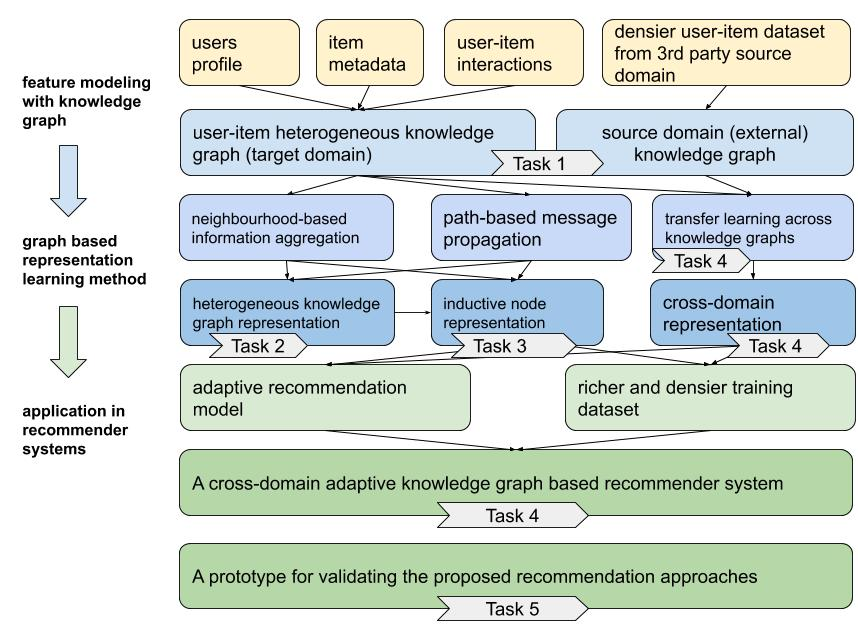
\includegraphics[width=0.98\textwidth]{figs/framework_overview.jpg}
    \caption{framework overview}\label{fig:framework}
\end{figure*}

\subsection*{Task 1: Propose a recommendation framework to form a unified knowledge graph to accommodate both user/item profile and interactions}

For the first task, we form the user-item heterogeneous knowledge graph by unifying user profile, item feature, as well as user-item interactions into a single unified heterogeneous graph.

First, we use side information to crate user and item knowledge graphs. The nodes inside graph can either be item or item features as entities based on data exploration and analytics. Same process applies to the user side, i.e. profile information, such as age, gender, etc. In the end, we would have 2 heterogeneous knowledge graphs, based on users and items perspectively as illustrated as G1 and G2 in Fig \ref{fig:meta_task}.
Consequently, we treat user-item interactions as a bipartite graph (as G3 Fig \ref{fig:meta_task}). As a result, user and item nodes in G1 and G2 are now connected by G3 via "interaction" edges. After this step, we get a unified heterogeneous knowledge graph which contains both user/item feature information as well as interactions.


\begin{figure*}[!ht]
    \centering
    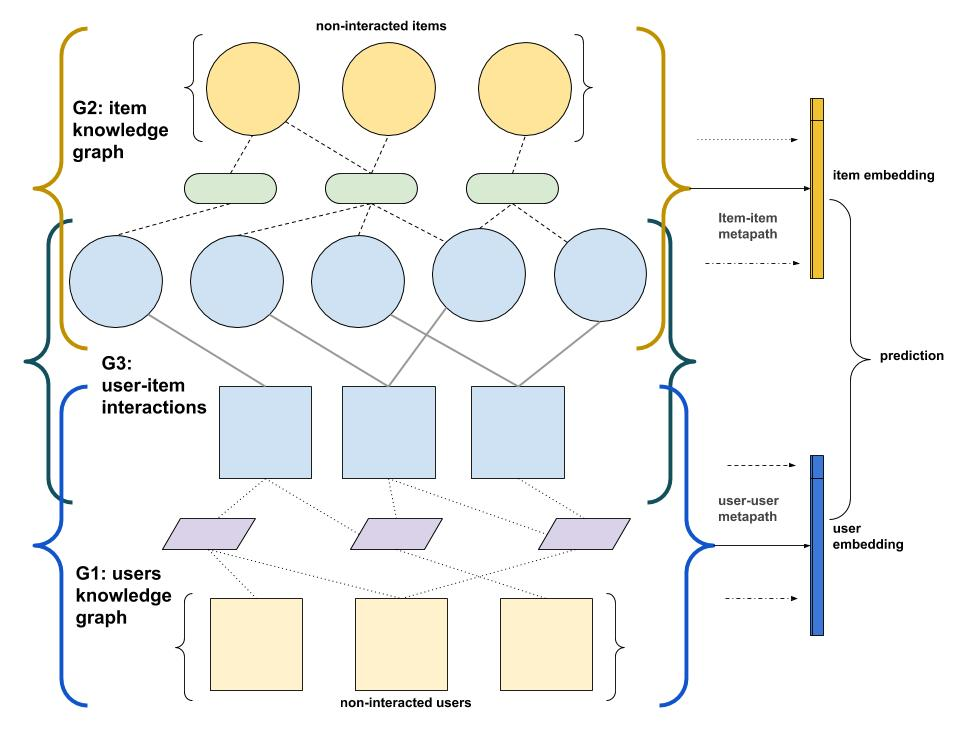
\includegraphics[width=0.98\textwidth]{figs/meta-embedding.jpg}
    \caption{meta-path based interactions via heterogeneous knowledge graph}\label{fig:meta_task}
\end{figure*}

The rich semantic heterogeneous graph structure enables the new data coming to establish relationship via different node and edge types, which also allowing information to be propagated and aggregated through different pathways. 
Intuitively, the node-to-node distance and neighborhood structural comparisons can be both used in measuring user/item similarity for existing or new nodes. In task 3 and 4, we would further explore this property to overcome cold start problems and improve recommendation model adaptiveness


\subsection*{Task 2: Build a recommendation method to leverage user/item representation with heterogeneous knowledge graph}

Following to task 1, incorporating the rich heterogeneous knowledge graph into recommender system is not a straight forward process. Most recommender models are only capable of processing structured data. The aim of this task is to transforming node into latent representation through nodes' neighborhood propagation for recommender system to use.

In addition to using direct connections, in this task, we adopts experts knowledge into representation modeling process by defining meta-path connections between nodes. As a result, we now can establish indirect user-item connections based on the heterogeneous knowledge graph. For example, \textit{User - Movie} interaction, can be extend to \textit{User - Movie1 - Actor - Movie2}. Consequently, collaborative filtering based recommendation approach can be benefited from the denser datasets.

Consequently, high-order connectivity with in heterogeneous knowledge graph is included as part of node representation learning process. So that, side information such as user demographics, item feature representation and node structural information can be learnt and transform into feature vectors holistically for the representative model.
Another added benefit of meta-path approach is reducing bias, which happens commonly in early stage of recommender systems. i.e. When data is not sufficiently available to represent a complete user/item distribution.

Lastly, we propose a recommendation framework that incorporates above representation approach. By leveraging CF information and path-based similarity within the heterogeneous knowledge graph. As illustrated in Fig \ref{fig:meta_task}, both interacted and non-interacted user/item entities now can participated into recommender model training.

\subsection*{Task 3: Build a adaptive representation method that is capable of working with unseen user/item data input}

So far, task 1 and task 2 try to alleviate data sparsity problem by forming heterogeneous knowledge graph and establish indirect connections via meta-path. However, our recommendation model is still limited to a static recommendation. i.e. The model is only capable of making predictions on data presented during training phase.

\begin{figure*}[!ht]
    \centering
    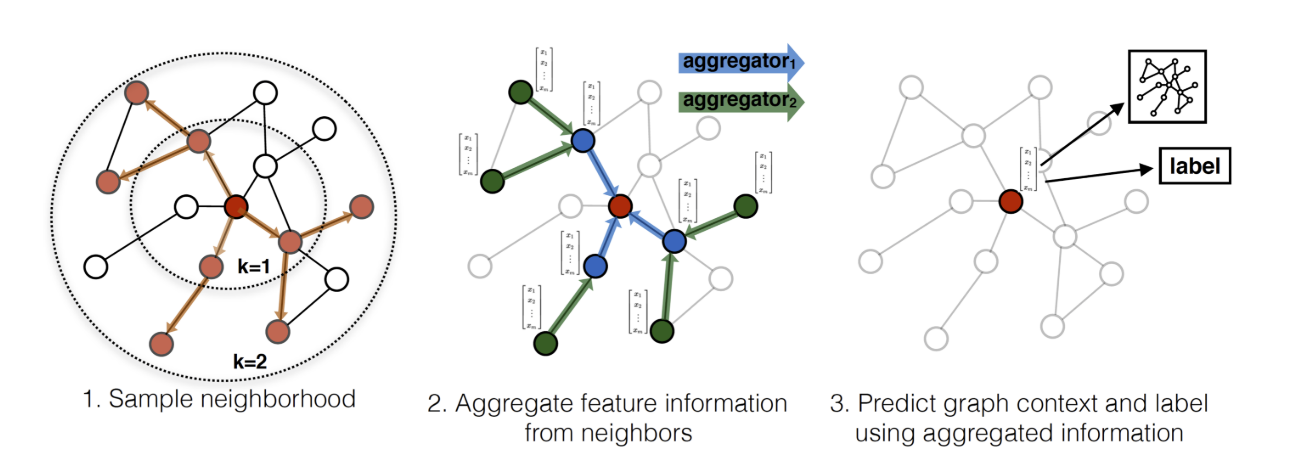
\includegraphics[width=0.95\textwidth]{figs/sagegraph.png}
    \caption{sage graph embedding}\label{fig:sagegraph}
\end{figure*}

In order to solve the challenge, the graph convolution network based embedding approach has shown promising results on classification and link prediction problems. \citet{hamilton2017inductive} uses function that generates embeddings by sampling and aggregating features from node neighbors, as shown in Fig. \ref{fig:sagegraph}. In this task, we extend the neighborhood sampling by taking part different meta-path connections into this task. This results a extended message propagation and aggregation rules to sample neighborhood and layers within the knowledge graph. Intuitively, different node relationships would be taken part in the embedding process.

Subsequently, attention approach can be employed. As illustrated in Fig. \ref{fig:gat}, similar to the graph attention network (GAT) approach \citep{velivckovic2017graph}, we apply multi-headed attention mechanisms, which learns different attention coefficients on its neighborhood nodes. The neighborhood nodes here are nodes either directly or indirectly connected via path and meta-paths. Subsequently, the later learnt attention coefficients weights can be used to explain the importance of different meta-paths, which leads to better model interoperability.

\begin{figure*}[!ht]
    \centering
    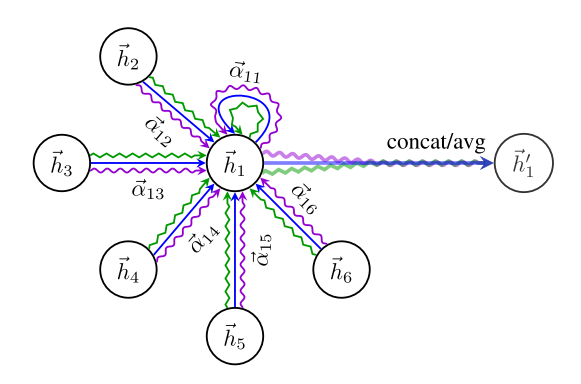
\includegraphics[width=0.6\textwidth]{figs/gat.png}
    \caption{graph attention network}\label{fig:gat}
\end{figure*}

We expect the end result will introduce a general inductive approach, which can efficiently generate node embeddings for unseen data that is not initially included during training.
Experiment will be conducted on different propagation and aggregator approach for node neighborhood sampling. We measure and compare different pooling rules and attention mechanism for the inductive learning step.

At a high level, this task solves the limitations by inductively generate node embeddings for new data points were not present during training for recommendation predictions. as a result, in the end the final recommendation model are more adaptive to new data input, and more capable of handling prediction in cold start settings.


\subsection*{Task 4: Define a recommendation method that leverage inductive representation}
In this task, we aim to optimize node representation inside knowledge graph jointly with collaborative user-item interactions for recommendation objectives.
Based on the findings from task 3, we apply earlier defined propagation rule and aggregator method under following objective function as:

\begin{equation}
    Loss=\min{(L_\text{KGE}+L_\text{FM}+\lambda\|\theta\|^2_2)}
\end{equation}

Where $L_\text{KGE}$ is the optimization target for representation embedding in knowledge graph. Next, we will experiment on different loss option for optimizing recommendation problem. For example, the entity representation can be optimise based on translation principle \citep{lin2017learning}.

\begin{equation}
    L_\text{KGE}=\sum{(h,r,t^+,t^-)} -ln_{sigmoid}(g(h,r,t^-)-g(h,r,t^+))
\end{equation}

While $g(h,r,t)$ is the projected probability from entity $h$ to target entity $t$ propagated via relationship $r$. $^+,^-$ stands for positive and negative samples. Accordingly $L_\text{FM}$ is the BPR \citep{rendle2012bpr} loss for optimizing recommendation objectives.
\begin{equation}
    L_\text{FM} = L_\text{BPR}=\sum{(u,i^+,i^-) \in G_{u,i}} -ln_{sigmoid}(y(u,i^+)-y(u,i^-))
\end{equation}
Where y(u,i) commonly stands for user-item dot product, Intuitively, the its result can be regarded as similarity score.

Lastly, regularization is applied on $\theta$ as model parameters.

Consequently, the trained model entity representation would tailored toward the recommendation objective in a end-to-end fashion.

Experiment and evaluation will be con ducted on multiple data conditions, such as sparse dataset, cold stat, zero interaction settings to compare and measure the effectiveness of proposed methods.


\subsection*{Task 5: Develop a knowledge transfer method to improve target domain data sparsity by leveraging source knowledge graph}

In this task, we are going to focus more on transferring knowledge from a different domain, where similar but more abundant information can be learnt and adapted from source domain to target domain for improving both entity representation and recommendation objectives. The research and experiments inside this task will be conducted on 2 different approaches:

\subsubsection*{Matrix-based FM method for cross-domain knowledge transfer}
Matrix-based FM method projects nodes and its neighborhood as one-hot encoding from both source and target knowledge graph into a single matrix. This way, we can treat the matrix containing domain-shared information, such as overlapped user or items. Following up, factorization machine approach is applied on top of the derived matrix. Hence embedding vector can be learnt as $FM(x) = v_x \in R^k$, where $k$ is the vector dimension. Knowledge graph based embedding, which was discussed in task 2 and 3 will be applied here for learning source and target domain-specific representations as $KGE(x)$.
Lastly, concatenation is applied, as, intuitively to combine both domain-shared and domain-specific representations into a single vector.
Additionally, a share $MLP$ function can be applied on both $FM(x)$ and $KGE(x)$ during training phrase. so, the final representation can be denoted as $v_x = [MLP(MF(x));MLP(KEG(x))]$, where $";"$ stand for the concatenation of two node representations.

\subsubsection*{GANs-based method for cross-domain knowledge transfer}
Adversarial domain adaptation technique is another approach we will experiment on transferring knowledge across 2 different domains.
First, we identify common entities, for example shared users or items or their related metadata (such as, item labels, demographics, etc.), to establish connections between source and target domain, and consequently unifying the target and source domain into a single knowledge graph.
Again, knowledge graph embedding will be used for node representation on the unified knowledge graph. Next, a 2 players minimax game are designed for alignment between target and source domains. i.e. a critic will be used for distinguish domain origin based on node representation or interaction connections. A more detail example can be seen in task 6.


\subsection*{Task 6: Develop a cross-domains recommender systems based on heterogeneous knowledge graph}

For this task, we extend recommendation model from single domain to multiple domains, in order to further explore on domain adaptation ability by leverage 2 or more knowledge graphs.

Similarly to single domain, we establish richer user-item connections across the source and target domains. Further, common cross-domain entities as described in task 5 can now serve as bridges for unifying and transferring information between 2 knowledge graphs.
For example, when target and source domains shares a common sub-section of users.

Following GANs intuition, we can introduce domain classifier D as critic, a binary classifier, to predict the origin of positive item sample. i.e. is the item belonged to source or target domain based on its representation vector as classifier input. Intuitively, cross graphs node representation and D now can be regarded as 2 players minimax game. It is expected node representation become domain-invariant when reaching equilibrium, i.e. knowledge is transfers across domains, that leads the source and target domain to be aligned. The domain alignment loss can be defined as:

\begin{equation}
    L_\text{DA}(e_s,e_t)=E_{e \in D_s}[log(1-D(e_s))] + E_{e \in D_t}[log(D(e_t))]
\end{equation}

Finally we adjust our cross-domain recommendation objective to as following:

\begin{equation}
    Loss=\min{(L_\text{DA}+L_\text{FM}+\lambda\|\theta\|^2_2)}
\end{equation}



\subsection*{Task 7: Build a prototype for validating the proposed recommendation approaches}

The research will be verified from two aspects:
First, verify knowledge graph based recommendation approach using public datasets, such as DBLP Citation Networks, MovieLens data sets. Similarity measure as well as adaptiveness are the core parts of this research, each aspects will be verified accordingly.
Second, the recommendation approach will be used in a real world data sets for solving industry problems. Such as, tourism , job posting and real estate listings where suffers from constant cold start problems. Experiments will be used to further test the effectiveness of the proposed method.



\section{Ethics and risk consideration}
According to ``HREC Guidelines for Undergraduate and Postgraduate Student'', this research does not need HREC approval.
The theory, algorithms and software development are not involved human and private data. Therefore, there is no ethical issue.

\section{Research schedule and progress to date}
 

\begin{table}[h!]
    \begin{tabular}{ |p{2cm}|p{6cm}|p{4cm}|}
     \hline
        Schedule & Research Stage & Progress \\
     \hline
        \rowcolor{gray}
        Aug 2018  & Stage 1. Comprehensive literature review progress  & completed  \\
        \hline
        \rowcolor{gray}
        Aug 2019  & Stage 2. Identify research questions and objectives  & completed  \\
        \rowcolor{gray}
        & Stage 3. Propose a knowledge graph based approach to accommodate interactions and side information & The result of this stage has been published in a conference paper. \\
        \hline
        \rowcolor{lightgray}
        Aug 2020  & Stage 4. Propose a representation method in heterogeneous knowledge graph for enhanced recommendation model training & The results has been published in a conference paper  \\
        \rowcolor{lightgray}
        & Stage 5. Propose a recommendation method that is adaptive to unseen data points  & Working on methods development \\
        \hline
        Aug 2021  & Stage 6. Develop a knowledge graph transfer learning method to improve target domain data sparsity & \\
        \hline
        Aug 2022  & Stage 7. Develop a cross-domains recommender systems framework based on heterogeneous knowledge graph  & \\
        & Stage 8.  A case study for validating the proposed recommendation approaches  & \\
        \hline
        Aug 2023 & Stage 9. Writing dissertation & \\
      \hline
     \end{tabular}
\end{table}

\bigskip
\bigskip
Based on the research, the following papers have been published:
\begin{enumerate}
    \item Zhang, D., Zhang, Q., Zhang, G. \& Lu, J., 2019,  ‘FreshGraph :  A spam-aware recommender system for cold start problem’, International Conference on Intelligent Systems and Knowledge Engineering (ISKE).
    \item Zhang, D., Zhang, Q., Zhang, G. \& Lu, J., 2020, ‘Recommender systems with heterogeneous information network for cold start items’, International Conference on Intelligent Systems and Knowledge Engineering (FLINS).
\end{enumerate}
 


\renewcommand{\bibname}{References}
\bibliography{reference.bib}

\clearpage

\end{document}
